\documentclass[12pt]{article}
%Gummi|065|=)
\usepackage{amsmath, amsfonts, amssymb}
\usepackage[margin=0.5in]{geometry}
\usepackage{xcolor}
\usepackage{graphicx}

% zeta functions of cubic fields

%\usepackage{pifont}
\usepackage{amsmath}

\newcommand{\off}[1]{}
\DeclareMathSizes{20}{30}{20}{18}

\newcommand{\two }{\sqrt[3]{2}}
\newcommand{\four}{\sqrt[3]{4}}
\newcommand{\red}{\begin{tikz}[scale=0.25]
\draw[fill=red, color=red] (0,0)--(1,0)--(1,1)--(0,1)--cycle;\end{tikz}}
\newcommand{\blue}{\begin{tikz}[scale=0.25]
\draw[fill=blue, color=blue] (0,0)--(1,0)--(1,1)--(0,1)--cycle;\end{tikz}}
\newcommand{\green}{\begin{tikz}[scale=0.25]
\draw[fill=green, color=green] (0,0)--(1,0)--(1,1)--(0,1)--cycle;\end{tikz}}

\newcommand{\sq}[3]{\draw[#3] (#1,#2)--(#1+1,#2)--(#1+1,#2+1)--(#1,#2+1)--cycle;}

\usepackage{tikz}

\newcommand{\susy}{{\bf Q}}
\newcommand{\RV}{{\text{R}_\text{V}}}

\title{Scratchwork: Prime Numbers in $\mathbb{Z}(\sqrt{2})$ or $\mathbb{Z}[i]$}
\date{}
\begin{document}

%\fontfamily{qag}\selectfont \fontsize{12.5}{15}\selectfont

\sffamily

\maketitle

\noindent Let's start by drawing a grid: \\ \\
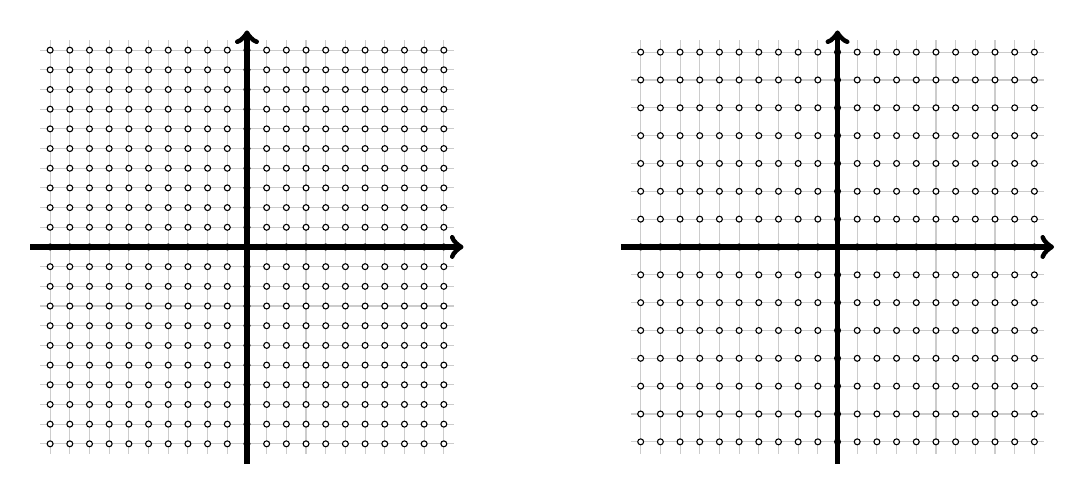
\begin{tikzpicture}[scale=0.25]

\foreach \a in {-10,...,10}{
	\draw[color=black!20!white] (\a,-10.5)--(\a,10.5);
	\draw[color=black!20!white] (-10.5,\a)--(10.5,\a);
}


\foreach \a in {-10,...,10}{
	\foreach \b in {-10,...,10}{
		\draw[fill=white] (\a,\b) circle (0.15);
	}
}

\draw[->, line width=2] (-11,0)--(11,0);
\draw[->, line width=2] (0,-11)--(0,11);

\begin{scope}[xshift=30cm]
\foreach \a in {-10,...,10}{
	\draw[color=black!20!white] (\a,-10.5)--(\a,10.5);
}

\foreach \a in {-7,...,7}{
	\draw[color=black!20!white] (-10.5,1.414*\a)--(10.5,1.414*\a);
}


\foreach \a in {-10,...,10}{
	\foreach \b in {-7,...,7}{
		\draw[fill=white] (\a,\b*1.414) circle (0.15);
	}
}

\draw[->, line width=2] (-11,0)--(11,0);
\draw[->, line width=2] (0,-11)--(0,11);
\end{scope}

\end{tikzpicture} \\ 
The first grid represents $\mathcal{O}_K = \mathbb{Z}[i]$ where $K = \mathbb{Q}(\sqrt{-1}) \simeq \mathbb{Q}[x]/(x^2 + 1)$. \\ \\
The second grid represents $\mathcal{O}_K = \mathbb{Z}[\sqrt{2}]$ where $K = \mathbb{Q}(\sqrt{2}) \simeq \mathbb{Q}[x]/(x^2 - 2)$. \\ \\
Our goal is to strip away these grid to obtain the set of prime numbers in both settings.  These are well-studied problems with detailed algebraic solutions, the goal is to solve these examples for ourselves. \\ \\
In the case of $\mathbb{Z}[i]$ all that seems to matter is the first quadrant.  The group action $\times \sqrt{-1}$ is, for the moment a $90^\circ$ rotation counterclockwise.  We have that $(1) < (1+i) < (2) < (1+2i) $ with nothing in between.  These are \textbf{ideals} and we have $(1+i) = (1-i)$.  We have that $(2)$ is \textbf{not}
prime.  $(2) = (1+i)^2 = (1+i)(1-i)$ \\ \\
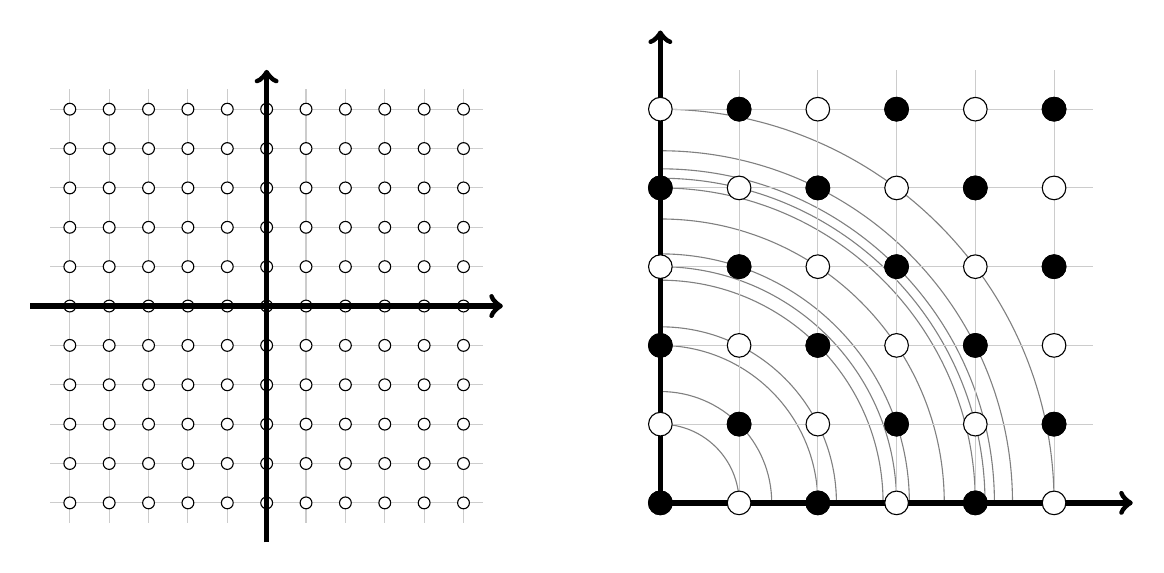
\begin{tikzpicture}[scale=0.5]

\foreach \a in {-5,...,5}{
	\draw[color=black!20!white] (\a,-5.5)--(\a,5.5);
	\draw[color=black!20!white] (-5.5,\a)--(5.5,\a);
}


\foreach \a in {-5,...,5}{
	\foreach \b in {-5,...,5}{
		\draw[fill=white] (\a,\b) circle (0.15);
	}
}

\draw[->, line width=2] (-6,0)--(6,0);
\draw[->, line width=2] (0,-6)--(0,6);


\begin{scope}[xshift=10cm, scale=2, yshift=-2.5cm]

\foreach \r in {  0.        ,   1.        ,   1.41421356,   2.        ,
         2.23606798,   2.82842712,   3.        ,   3.16227766,
         3.60555128,   4.        ,   4.12310563,   4.24264069,
         4.47213595,   5.    }
{

	\draw[color=black!50!white] (\r,0) arc (0:90:\r);

}

\foreach \a in {0,...,5}{
	\draw[color=black!20!white] (\a,0)--(\a,5.5);
	\draw[color=black!20!white] (0,\a)--(5.5,\a);
}

\draw[->, line width=2] (0,0)--(6,0);
\draw[->, line width=2] (0,0)--(0,6);




\foreach \a in {0,...,5}{
	\foreach \b in {0,...,5}{
		\draw[fill=white] (\a,\b) circle (0.15);
	}
}





\draw[fill=black] (0,0) circle (0.15);
\draw[fill=black] (0,2) circle (0.15);
\draw[fill=black] (1,1) circle (0.15);
\draw[fill=black] (2,0) circle (0.15);
\draw[fill=black] (0,4) circle (0.15);
\draw[fill=black] (1,3) circle (0.15);
\draw[fill=black] (2,2) circle (0.15);
\draw[fill=black] (3,1) circle (0.15);
\draw[fill=black] (4,0) circle (0.15);
\draw[fill=black] (1,5) circle (0.15);
\draw[fill=black] (2,4) circle (0.15);
\draw[fill=black] (3,3) circle (0.15);
\draw[fill=black] (4,2) circle (0.15);
\draw[fill=black] (5,1) circle (0.15);
\draw[fill=black] (3,5) circle (0.15);
\draw[fill=black] (4,4) circle (0.15);
\draw[fill=black] (5,3) circle (0.15);
\draw[fill=black] (5,5) circle (0.15);

\end{scope}


\end{tikzpicture}\\
We know that $(1+2i) \big| (5)$ and we even have that $5 = (1+2i)\times(1-2i)$.  At first glance $(3) \approx (1 + 2i)\approx 2 \times (1+i)$. \\
The algebra is slightly misleading here since it makes things that are close together (approximate over $\mathbb{R}$) look very distant.  This could be useful to us. \\\\
\textbf{Ex.} $(1+2i) \stackrel{?}{=} (1-2i)$
\end{document}